%
\documentclass[twoside]{article}
% \linespread{0.99}
%
%\usepackage{float}
\setlength{\textfloatsep}{11pt}
\usepackage{floatrow}
\usepackage{ifthen}
\usepackage{xspace}
\usepackage[T1]{fontenc}
\usepackage[OT1]{eulervm}
\usepackage[dvipsnames]{xcolor}
\usepackage{ftnright}
\usepackage{sepfootnotes}
\ifthenelse{\NOT\isundefined{\draft}\OR\NOT\isundefined{\final}}{
    \usepackage{acro}
    \acsetup{
        list-style     = tabular,
        single         = true ,
        sort           = true ,
        cite-cmd       = \citep ,
        group-citation = true ,
        group-cite-cmd = \citealp
    }
}{
    \usepackage{acro}
    \acsetup{
        list-style     = tabular,
        single         = true ,
        sort           = true ,
        cite-cmd       = \citep ,
        group-citation = true ,
        group-cite-cmd = \citealp
    }
    %\newcommand\ac[1]{#1}
    %\newcommand\acs[1]{#1}
    %\newcommand\acp[1]{#1}
    %\newcommand\acl[1]{#1}
    %\newcommand\aclp[1]{#1}
    %\newcommand\acf[1]{#1}
    %\newcommand\acfp[1]{#1}
}
\usepackage[colorlinks=true,
            linkcolor=Blue,
            urlcolor=Blue,
            citecolor=Blue]{hyperref}
\usepackage{ragged2e}
\usepackage{microtype}
\usepackage{dirtytalk}
\usepackage{pdflscape}
\usepackage{afterpage}
\usepackage{fancyvrb}
\usepackage{placeins}
\usepackage{csquotes}
\usepackage{filecontents}
\usepackage{url}            % simple URL typesetting
\usepackage{booktabs}       % professional-quality tables
\usepackage{nicefrac}       % compact symbols for 1/2, etc.
\usepackage{microtype}
\usepackage{graphicx}
\usepackage{nicefrac}
\usepackage[tableposition=top]{caption}
\usepackage[position=top]{subcaption}
% \usepackage[round]{natbib}
% \renewcommand{\bibname}{References}
% \renewcommand{\bibsection}{\subsubsection*{\bibname}}
\usepackage[backend=biber, style=authoryear-comp, maxcitenames=1,
            natbib=true, bibencoding=utf8, hyperref=true,
            abbreviate=true, firstinits=true,
            %sorting=ynt,
            backref=true, citetracker=true]{biblatex}
%\usepackage[textwidth=2.0cm, textsize=scriptsize]{todonotes}
% modification to natbib citations
\VerbatimFootnotes
\usepackage[export]{adjustbox}
\usepackage{pgf}
\usepackage{pgfplots}
\usepackage{tikz}
\usetikzlibrary{pgfplots.groupplots}
\usetikzlibrary{external}
\usetikzlibrary{quotes,angles}
\usetikzlibrary{cd}
\usetikzlibrary{matrix}
\usetikzlibrary{calc}
\makeatletter
\tikzset{%
    column sep/.code=\def\pgfmatrixcolumnsep{\pgf@matrix@xscale*(#1)},
    row sep/.code   =\def\pgfmatrixrowsep{\pgf@matrix@yscale*(#1)},
    matrix xscale/.code=%
    \pgfmathsetmacro\pgf@matrix@xscale{\pgf@matrix@xscale*(#1)},
    matrix yscale/.code=%
    \pgfmathsetmacro\pgf@matrix@yscale{\pgf@matrix@yscale*(#1)},
    matrix scale/.style={/tikz/matrix xscale={#1},/tikz/matrix yscale={#1}}}
\def\pgf@matrix@xscale{1}
\def\pgf@matrix@yscale{1}
\makeatother
\pgfplotsset{compat=newest}
\usepackage{amsmath, amsthm, amssymb, amsfonts, bbm}
\usepackage[american]{babel}
\usepackage{braket}
\usepackage{colonequals}
\usepackage{thmtools}
\usepackage{nameref}
\usepackage[capitalise]{cleveref}
\usepackage{mathtools}
\usepackage[algo2e, ruled, linesnumbered]{algorithm2e}
\usepackage{tablefootnote}
\usepackage{breqn}
\usepackage{commands}
\usepackage{paralist, enumitem}
\usepackage{multicol}
\usepackage{multirow}
\usepackage{booktabs}
%\usepackage{tabularx}
\usepackage{ltablex}
\usepackage{chngpage}
%\usepackage{threeparttablex}
\usepackage[mathscr]{eucal}
\usepackage{floatflt}
\setlength{\extrarowheight}{3pt}
\newcommand{\tableheadline}[1]{\multicolumn{1}{c}{\spacedlowsmallcaps{#1}}}
\newcommand{\myfloatalign}{\centering}
\newcommand{\theHalgorithm}{\arabic{algorithm}}
\usepackage[symbol]{footmisc}
%
\creflabelformat{equation}{#2(\textup{#1})#3}
%
% \usepackage[margin=1in]{geometry}
% \usepackage{times}
%
\usepackage[accepted]{aistats2019}
% If your paper is accepted and the title of your paper is very long,
% the style will print as headings an error message. Use the following
% command to supply a shorter title of your paper so that it can be
% used as headings.
%
%\runningtitle{I use this title instead because the last one was very long}

% If your paper is accepted and the number of authors is large, the
% style will print as headings an error message. Use the following
% command to supply a shorter version of the authors names so that
% they can be used as headings (for example, use only the surnames)
%
%\runningauthor{Surname 1, Surname 2, Surname 3, ...., Surname n}
%
\addbibresource{references.bib}
\floatsetup[table]{capposition=top}
%

% \renewcommand\bibliographytypesize{\small}
\begin{document}
%
\begin{poster}{
    eyecatcher=true,
    background=plain,
    bgColorOne=black!5,
    headershade=plain,
    headerColorOne=black!10,
    headerFontColor=black,
    headershape=rectangle,
    headerfont=\LARGE\bf,
    textborder=none,
    headerborder=none,
    boxshade=plain,
    boxColorOne=white,
    columns=2,
    % colspacing=3cm,
}
{
% \includegraphics[height=10ex]{inria_logo.jpg}

\includegraphics[height=10ex]{logos/tpt.pdf}

\includegraphics[height=10ex]{logos/x.jpg}
}
{
Infinite Task Learning in RKHSs
}
{
\def\PARISTECH{\unskip$^{\dagger}$}
\def\CMAP{\unskip$^{\star}$}
\def\LDS{\unskip$^{\clubsuit}$}
\def\LIP{\unskip$^{\spadesuit}$}
  \large
    R. Brault\LDS,
    A. Lambert\PARISTECH,
    Z. Szab{\'o}\CMAP,
    M. Sangnier\LIP,
    F. d'Alch\'{e}-Buc \PARISTECH\\
   \mbox{$\clubsuit$ L2S,  Centrale-Sup{\'e}lec.}
   \mbox{$\dagger$ LTCI, T\'el\'ecom ParisTech.}
   \mbox{$\star$ CMAP,  {\'E}cole Polytechnique.}
   \mbox{$\spadesuit$ LIP6, Sorbonne Universit\'{e}.}
}\par
%
%
%%%%%%%%%%%%%%%%%%%%%%%%%%%%%%%%%%%%%%%%%%%%%%%%%%%%%%%%%%%%%%%%%%%%%%
\begin{posterbox}[name=parametrized_tasks, column=0]{A Kind of Multi-Output Regression}
Risk minimization for function-valued regression:
\begin{itemize}
  \item $\mcX$ input space ($\reals^d$), $\Theta$ parameter space ($\subset \reals$), $\mcY$ output space ($\subset \reals$).
  \item Hypothesis space $\hypothesisspace \subset \functionspace{\inputspace}{
    \functionspace{\hyperparameterspace}{\outputspace}}$ \emph{, i.e.} ~$h(x) \in \functionspace{\hyperparameterspace}{\outputspace}$.
  \item Parametrized cost $v \colon \Theta \times \mcY \times \mcY \to \reals$.
  \item Local loss $
      \cost(y, h(x)) \defeq \displaystyle\int_{\hyperparameterspace}
      \hcost(\hyperparameter,y,
      h(x)(\hyperparameter))d\mu(\hyperparameter)$.
\end{itemize}
Minimizing population risk:
\begin{align}\label{equation:h-objective}
    \argmin_{h\in \hypothesisspace } R(h) \defeq \expectation_{X,Y} \left[ \cost(Y,
    h(X))\right].
\end{align}
\begin{center}
  $\Rightarrow$ Extension of Multi-Task Learning to an infinite number of tasks \citep{takeuchi2013parametric}.
\end{center}
\end{posterbox}
%%%%%%%%%%%%%%%%%%%%%%%%%%%%%%%%%%%%%%%%%%%%%%%%%%%%%%%%%%%%%%%%%%%%%%
\begin{posterbox}[name=examples,below=parametrized_tasks, column=0]{Two examples}
  \paragraph{\ac{QR}:}
  Given $X,Y \in \mcX \times \mcY$ random variables, estimate the quantile
  function of the conditional distribution $\probability_{Y|X}$:
  \begin{align} \label{definition:quantile}
    q(x)(\theta) = \inf \left \{  t \in \mcY,~ \probability_{Y|X=x}[Y \leq t] \geq \theta \right \} \quad \forall (x,\theta) \in \mcX \times (0,1).
  \end{align}
  Pinball loss:
  \begin{align} \label{pinball_loss}
     v(\hyperparameter,y, h(x)) = \abs{\hyperparameter - \indicator{\reals_{-}}(y - h(x))}\abs{y - h(x)}.
  \end{align}
  \begin{proposition}
    $q$ defined in (\ref{definition:quantile}) minimizes (\ref{equation:h-objective}) for
    the pinball loss (\ref{pinball_loss}).
  \end{proposition} \par
  \paragraph{\ac{CSC}:}
  Support Vector Machine with asymmetric loss function
  \begin{align*}
      v(\theta,y, h(x)) = \abs{\frac{\theta + 1}{2} -
      \indicator{\Set{-1}}(y)}\abs{1 - yh(x)}_{+}.
  \end{align*}
  The value of $\theta$ influences how the different classes are penalized.
\end{posterbox}
%%%%%%%%%%%%%%%%%%%%%%%%%%%%%%%%%%%%%%%%%%%%%%%%%%%%%%%%%%%%%%%%%%%%%%%
\begin{posterbox}[name=integral,below=examples, column=0]{Sampled Empirical Risk}
 Approximate expectation over $\probability_{X,Y}$ and $\int_{\Theta}$
 \begin{itemize}
   \item $(x_i,y_i)_{i=1}^n \stackrel{\text{i.i.d.}}{\sim} \probability_{X,Y}$
   \item $(\theta_j)_{j=1}^m \sim \mu$ (Quasi-Monte Carlo)
 \end{itemize}
 Sampled empirical risk:
 \begin{align*}
   \widetilde{R}_{\trainingset}(h) \defeq \frac{1}{nm} \sum_{i=1}^n \sum_{j=1}^m v(\theta_j,y_i,h(x_i)(\theta_j)).
 \end{align*}
 Regularized problem:
 \begin{align}\label{serproblem}
     \argmin_{h\in \hypothesisspace } \widetilde{R}_{\trainingset}(h) + \lambda  \Omega(h).
 \end{align}
\end{posterbox}
%%%%%%%%%%%%%%%%%%%%%%%%%%%%%%%%%%%%%%%%%%%%%%%%%%%%%%%%%%%%%%%%%%%%%%%
%%%%%%%%%%%%%%%%%%%%%%%%%%%%%%%%%%%%%%%%%%%%%%%%%%%%%%%%%%%%%%%%%%%%%%%
\begin{posterbox}[name=vv-rkhs,below=integral, column=0]{Vector-Valued RKHSs}
 Natural extension of RKHS for modelling outputs in any Hilbert space.
 \begin{itemize}
   \item $k_{\mcX} \colon \mcX \times \mcX \to \reals$ and
   $k_{\Theta} \colon \Theta \times \Theta \to \reals$ two scalar-valued kernels.
   \item Operator-valued kernel $K(x,z) = k_{\mcX}(x,z)I_{\mcH_{k_{\Theta}}}$
   associated to $\mcH_K$ a space of function-valued functions.
   \item $\hypothesisspace_K = \lspan \Set{K(\cdot,x)f |\enskip x \in
   \mcX,\enskip f \in \hypothesisspace_{k_{\hyperparameterspace}}} \cong \mcH_{k_{\mcX}} \otimes \mcH_{k_{\Theta}}$.
   \item Hilbert norm $\frac{1}{2}\norm{h}^2_{\mcH_K}$ as regularizer $\Omega(h)$.
\end{itemize}
\end{posterbox}
%%%%%%%%%%%%%%%%%%%%%%%%%%%%%%%%%%%%%%%%%%%%%%%%%%%%%%%%%%%%%%%%%%%%%%%
\begin{posterbox}[name=optimization,column=1]{Optimization}
\begin{proposition}[Representer]
 If $\forall \theta \in \Theta$, $v(\theta,\cdot,\cdot)$
 is proper lower semicontinuous with respect to its second argument, (\ref{serproblem})
 has a unique solution $h^* \in \mcH_K$, and $\exists$ $\left(\alpha_{ij}\right)_{i,j =
 1}^{n,m} \in \mathbb{R}^{n\times m}$ such that $\forall
 (x,\hyperparameter) \in \mcX \times \hyperparameterspace$
 \begin{align*}
     h^*(x)(\hyperparameter) &= \sum_{i=1}^{n} \sum_{j=1}^m \alpha_{ij}
     k_{\mcX}(x,x_i)
     k_{\hyperparameterspace}(\hyperparameter,\hyperparameter_j).
 \end{align*}
\end{proposition}
\begin{itemize}
  \item Solution shaped by $k_{\mcX}$ and $k_{\Theta}$ (Gaussian, Laplacian, ...)
  \item Infinite-dimensional problem $\Rightarrow$ size $n \cdot m$
  \item In practice, solved via smoothing $v$ + L-BFGS.
\end{itemize}
\end{posterbox}
%%%%%%%%%%%%%%%%%%%%%%%%%%%%%%%%%%%%%%%%%%%%%%%%%%%%%%%%%%%%%%%%%%%%%%%
\begin{posterbox}[name=excess_risk,below=optimization, column=1]{Excess Risk Guarantees}
  Framework of vv-RKHS allows for proper analysis \citep{kadri2015operator}, tradeoff $n/m$
  \begin{align*}\label{equation:excess_risk}
      \risk(h^*) \leq \widetilde{R}_{\mcS}(h^*) +
      \mathcal{O}_{\probability_{X,Y}} \left (\frac{1}{\sqrt{\lambda n}}
      \right ) + \mathcal{O} \left ( \frac{\log(m)}{\sqrt{\lambda}m} \right).
  \end{align*}
\end{posterbox}
%%%%%%%%%%%%%%%%%%%%%%%%%%%%%%%%%%%%%%%%%%%%%%%%%%%%%%%%%%%%%%%%%%%%%%%
\begin{posterbox}[name=numerical_ex,below=excess_risk, bottomaligned=vv-rkhs,column=1]{Numerical Experiments}
  \paragraph{\ac{QR}:} Continuous model $\Rightarrow$ new non-crossing constraint:
  \begin{align*}
    \widetilde{\Omega}_{\text{nc}}(h) =
    \frac{\lambda_{nc}}{nm}\sum_{i=1}^n\sum_{j=1}^m \abs{ -\frac{\partial
    h}{\partial \hyperparameter} (x_i)(\theta_j)}_+ .
  \end{align*}
  \begin{center}
      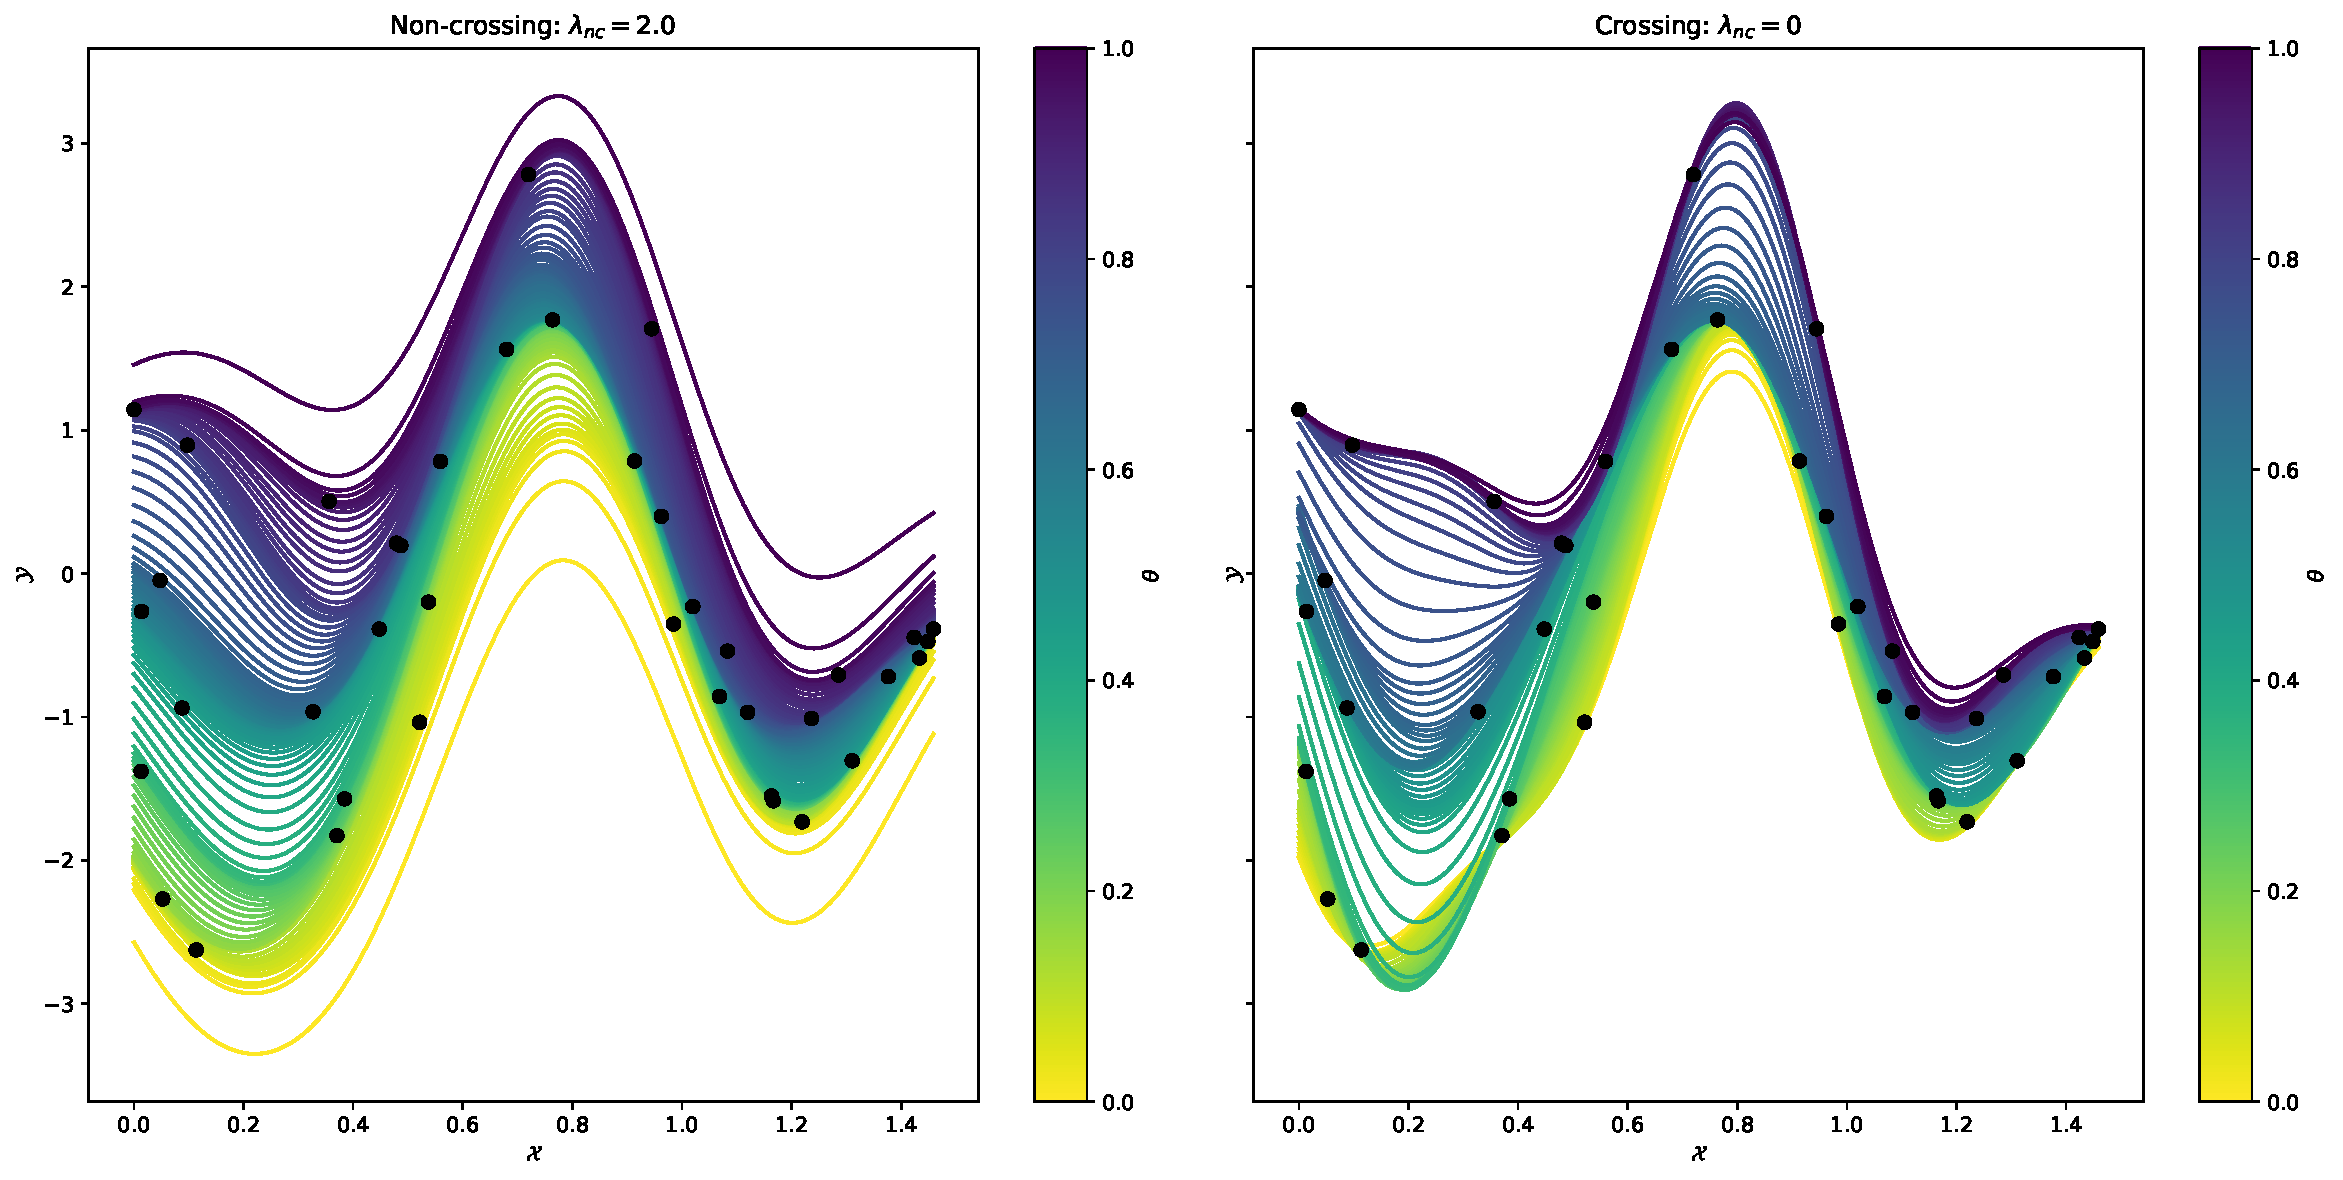
\includegraphics[width=0.8\textwidth]{fig/iqr_crossing.pdf}\\
      Left: strong
      non-crossing penalty ($\lambda_{\text{nc}}=2$). Right: no
      non-crossing penalty ($\lambda_{\text{nc}}=0)$.
      The plots show $100$
      quantiles of the continuum learned, linearly spaced
      between $0$ (yellow) and $1$ (purple).\\
  \end{center}
   \par
   \begin{center}
     $\Rightarrow$ Matches state of the art \citep{sangnier2016joint} on $20$ UCI datasets
   \end{center}
  \paragraph{\ac{CSC}:} Improved performance:
  \begin{center}
      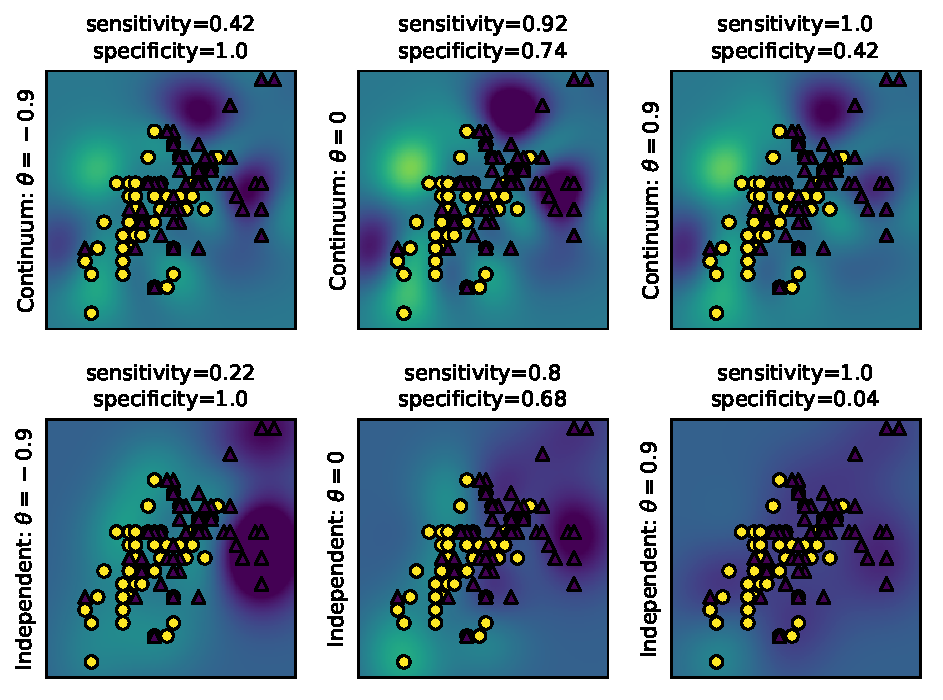
\includegraphics[width=0.7\textwidth]{fig/icsl_vs.pdf}\\
      Iris dataset. Top: infinite learning; bottom: independent learning
      for $\theta\in\Set{-0.9, 0, 0.9}$.\\
  \end{center}\par
  \begin{center}
    \emph{Code available:} https://bitbucket.org/RomainBrault/itl/
  \end{center}
\end{posterbox}
%%%%%%%%%%%%%%%%%%%%%%%%%%%%%%%%%%%%%%%%%%%%%%%%%%%%%%%%%%%%%%%%%%%%%%%
\begin{posterbox}[name=references, column=0,span=2,
                  headerColorOne=white,below=vv-rkhs
                  ]{\footnotesize{\normalfont This work was supported by the Labex DigiCosme (project ANR-11-LABEX-0045-
DIGICOSME) and the industrial chair Machine Learning for Big Data at T{\'e}l{\'e}com ParisTech.}}
\neutralisetitre
\bibliographystyle{plain}
{\footnotesize\setstretch{0.9}
% This work was funded by ERC Starting Grant SLAB ERC-YStG-676943 and the Chaire Machine Learning for Big Data of T\'el\'ecom ParisTech.
\vspace{-2mm}
\begin{thebibliography}{1}

% \bibitem{Fercoq_Gramfort_Salmon15}
% O.~Fercoq, A.~Gramfort, and J.~Salmon.
% \newblock Mind the duality gap: safer rules for the lasso.
% \newblock In {\em ICML}, pages 333--342, 2015.
% \\[-0.5cm]


\bibitem{takeuchi2013parametric}
Takeuchi, Ichiro and Hongo, Tatsuya and Sugiyama, Masashi and Nakajima, Shinichi.
\newblock Parametric task learning.
\newblock In \emph{NIPS}, pp.\  1358--1366, 2013.
\\[-0.5cm]

\bibitem{kadri2015operator}
Kadri, Hachem and Duflos, Emmanuel and Preux, Philippe and Canu, St{\'e}phane and Rakotomamonjy, Alain and Audiffren, Julien.
\newblock Operator-valued kernels for learning from functional response data.
\newblock  \emph{JMLR}, vol 16 pp 1--54, 2015.
\\[-0.5cm]


\bibitem{sangnier2016joint}
Sangnier, Maxime and Fercoq, Olivier and d'Alch{\'e}-Buc, Florence.
\newblock Joint quantile regression in vector-valued RKHSs.
\newblock In \emph{NIPS}, pp.\  3693--3701, 2016.


\end{thebibliography}
}
\end{posterbox}
%%%%%%%%%%%%%%%%%%%%%%%%%%%%%%%%%%%%%%%%%%%%%%%%%%%%%%%%%%%%%%%%%%%%%%%


\end{poster}
\end{document}
